\documentclass[12pt]{article}

% =========================================================
% PAQUETES
% =========================================================

\usepackage[utf8]{inputenc}
\usepackage[T1]{fontenc}
\usepackage[english]{babel}

\usepackage{amsmath}
\usepackage{amssymb}

\usepackage{geometry}
\geometry{
    letterpaper,
    left=2.5cm,
    right=2.5cm,
    top=2.5cm,
    bottom=2.5cm
}

% =========================================================
% TIKZ PARA DFA
% =========================================================

\usepackage{tikz}

\usetikzlibrary{
    automata,
    positioning,
    arrows.meta
}

\tikzset{
    >=Stealth,
    every state/.style={
        minimum size=1cm,
        inner sep=2pt
    }
}

% Quitar numeración de páginas en portada
\pagestyle{plain}

% =========================================================
% DOCUMENTO
% =========================================================

\begin{document}

% =========================================================
% PORTADA
% =========================================================

\begin{titlepage}

    \centering

    \vspace*{1.5cm}

    {\Large\textsc{Universidad de Costa Rica}\par}

    \vspace{0.7cm}

    {\large\textsc{Escuela de Ciencias de la Computación e Informática}\par}

    \vspace{0.8cm}

    {\large\textbf{CI-0146 Compilers}\par}

    % -----------------------------------------------------
    % TÍTULO
    % -----------------------------------------------------

    \vspace{2.5cm}

    \rule{0.88\textwidth}{0.6pt}

    \vspace{0.5cm}

    {\LARGE\textbf{Deterministic Finite Automata}\par}

    \vspace{0.5cm}

    \rule{0.88\textwidth}{0.6pt}

    % -----------------------------------------------------
    % PROFESOR Y ESTUDIANTES
    % -----------------------------------------------------

    \vspace{2.2cm}

    \noindent
    \begin{minipage}[t]{0.45\textwidth}
        \raggedright

        \textbf{Professor:}

        \vspace{0.25cm}

        Dr. Francisco J. Torres-Rojas

    \end{minipage}
    \hfill
    \begin{minipage}[t]{0.45\textwidth}
        \raggedleft

        \textbf{Students:}

        \vspace{0.25cm}

        José Guerra --- C33510\\
        Mario Cordero --- C22306\\
        Daniel Gómez --- C23310

    \end{minipage}

    % -----------------------------------------------------
    % FECHA
    % -----------------------------------------------------

    \vfill

    {\large
        \textbf{Delivery date:} [October 19th, 2026]
    \par}

    \vspace{1.5cm}

\end{titlepage}

% =========================================================
% EJERCICIO 12
% =========================================================

\section*{Exercise 12}

\begin{center}
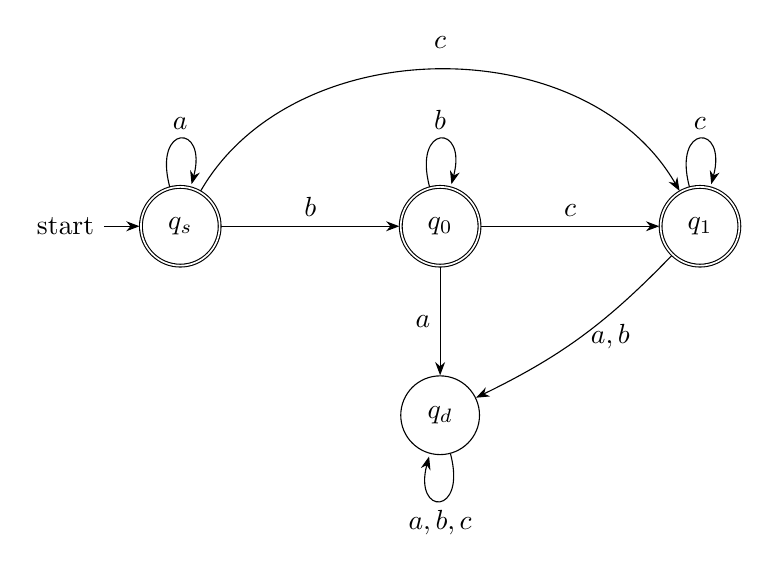
\begin{tikzpicture}[
    node distance=3.3cm,
    on grid,
    auto,
    >=Stealth
]

    % Estados
    \node[state, initial, accepting] (qs) {$q_s$};
    \node[state, accepting] (q0) [right=of qs] {$q_0$};
    \node[state, accepting] (q1) [right=of q0] {$q_1$};
    \node[state] (qd) [below=2.4cm of q0] {$q_d$};

    % Transiciones
    \path[->]
        (qs) edge[loop above] node{$a$} ()
             edge node[above]{$b$} (q0)
             edge[bend left=60] node[pos=0.5, above=4pt]{$c$} (q1)

        (q0) edge[loop above] node{$b$} ()
             edge node[above]{$c$} (q1)
             edge node[left]{$a$} (qd)

        (q1) edge[loop above] node{$c$} ()
             edge[bend left=10] node[right]{$a,b$} (qd)

        (qd) edge[loop below] node{$a,b,c$} ();

\end{tikzpicture}
\end{center}

\vspace{1cm}

% =========================================================
% EJERCICIO 13
% =========================================================

\section*{Exercise 13}

\begin{center}
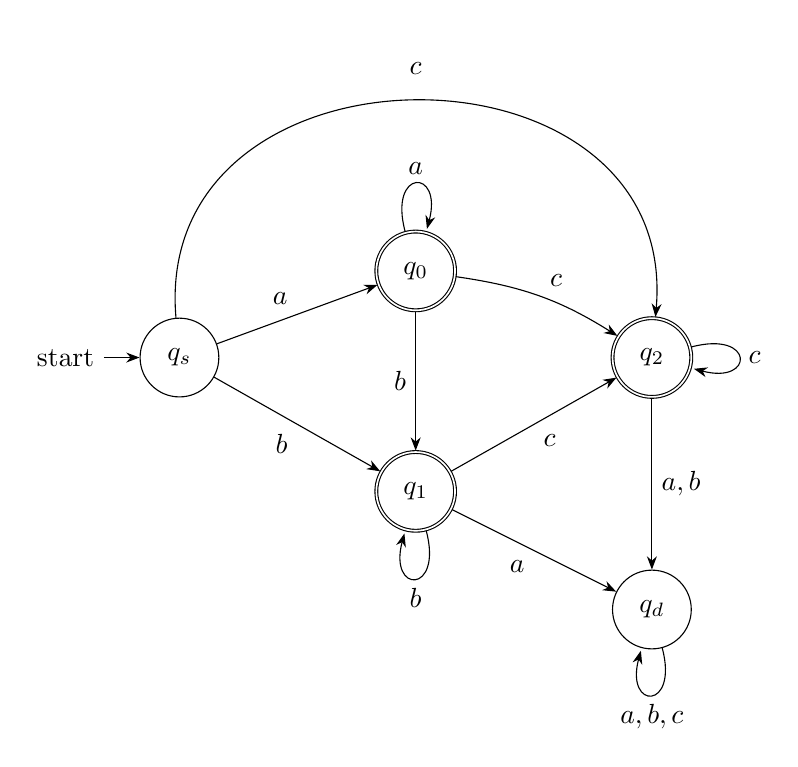
\begin{tikzpicture}[
    auto,
    >=Stealth
]

    % Estados
    \node[state, initial]   (qs) at (0,0)      {$q_s$};
    \node[state, accepting] (q0) at (3,1.1)    {$q_0$};
    \node[state, accepting] (q1) at (3,-1.7)   {$q_1$};
    \node[state, accepting] (q2) at (6,0)      {$q_2$};
    \node[state]            (qd) at (6,-3.2)   {$q_d$};

    % Transiciones
    \path[->]

        % Desde el estado inicial
        (qs)
            edge node[above left] {$a$} (q0)
            edge node[below left] {$b$} (q1)
            edge[
                out=95,
                in=85,
                looseness=1.55
            ]
            node[pos=0.5, above=6pt] {$c$} (q2)

        % Desde q0
        (q0)
            edge[loop above] node {$a$} ()
            edge node[left] {$b$} (q1)
            edge[bend left=12] node[above right] {$c$} (q2)

        % Desde q1
        (q1)
            edge[loop below] node {$b$} ()
            edge node[below right] {$c$} (q2)
            edge node[below left] {$a$} (qd)

        % Desde q2
        (q2)
            edge[loop right] node {$c$} ()
            edge node[right] {$a,b$} (qd)

        % Estado muerto
        (qd)
            edge[loop below] node {$a,b,c$} ();

\end{tikzpicture}
\end{center}

\vspace{1cm}

% =========================================================
% EJERCICIO 14
% =========================================================

\section*{Exercise 14}

\begin{center}
\begin{tikzpicture}[
    auto,
    >=Stealth
]

    % Estados
    \node[state, initial]   (qs) at (0,0)       {$q_s$};

    \node[state]            (q0) at (2.7,1.5)   {$q_0$};
    \node[state]            (q1) at (2.7,-1.5)  {$q_1$};

    \node[state, accepting] (q2) at (5.4,1.5)   {$q_2$};
    \node[state, accepting] (q3) at (5.4,-1.5)  {$q_3$};

    \node[state]            (qd) at (8,0)       {$q_d$};

    % Transiciones
    \path[->]

        % Desde el estado inicial
        (qs)
            edge node[above left] {$a$} (q0)
            edge node[below left] {$b$} (q1)

        % Desde q0
        (q0)
            edge node[above] {$a$} (q2)
            edge node[pos=0.3, below left] {$b$} (q3)

        % Desde q1
        (q1)
            edge node[above] {$b$} (q3)
            edge[
                out=-70,
                in=-90,
                looseness=1.80
            ]
            node[pos=0.50, below] {$a$} (qd)

        % Estado de aceptación superior
        (q2)
            edge[loop above] node {$a$} ()
            edge node[right] {$b$} (q3)

        % Estado de aceptación inferior
        (q3)
            edge[loop below] node {$b$} ()
            edge node[below right] {$a$} (qd)

        % Estado muerto
        (qd)
            edge[loop right] node {$a,b$} ();

\end{tikzpicture}
\end{center}

\vspace{1cm}

% =========================================================
% EJERCICIO 15
% =========================================================

\section*{Exercise 15}

\begin{center}
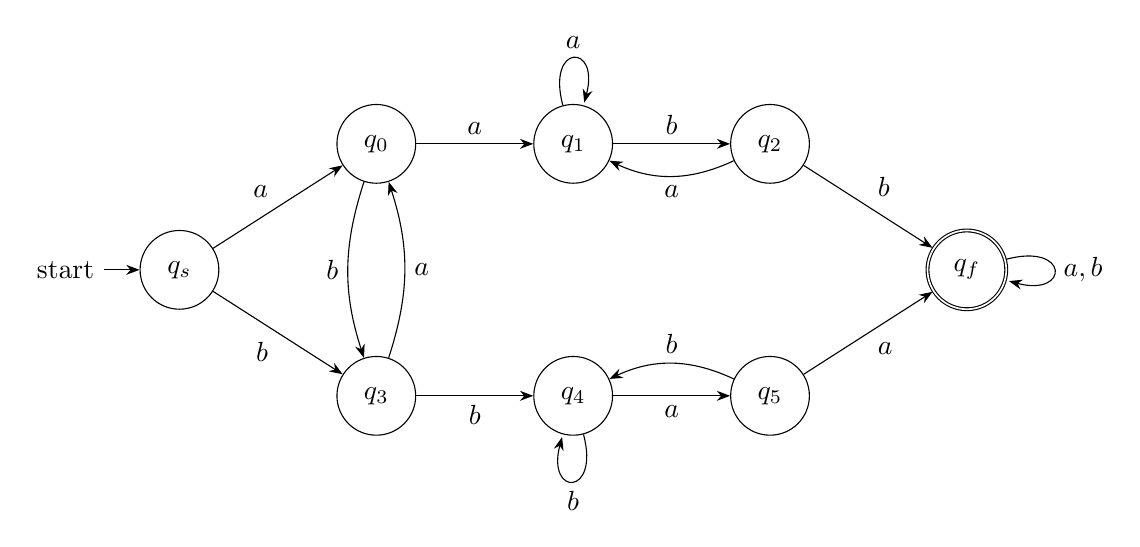
\begin{tikzpicture}[
    auto,
    >=Stealth
]

    % Estados
    \node[state, initial]   (qs) at (0,0)       {$q_s$};

    % Rama superior
    \node[state]            (q0) at (2.5,1.6)   {$q_0$};
    \node[state]            (q1) at (5,1.6)     {$q_1$};
    \node[state]            (q2) at (7.5,1.6)   {$q_2$};

    % Rama inferior
    \node[state]            (q3) at (2.5,-1.6)  {$q_3$};
    \node[state]            (q4) at (5,-1.6)    {$q_4$};
    \node[state]            (q5) at (7.5,-1.6)  {$q_5$};

    % Estado final
    \node[state, accepting] (qf) at (10,0)      {$q_f$};

    % Transiciones
    \path[->]

        % Desde el estado inicial
        (qs)
            edge node[above left] {$a$} (q0)
            edge node[below left] {$b$} (q3)

        % Rama superior
        (q0)
            edge node[above] {$a$} (q1)
            edge[bend right=18]
                node[left] {$b$} (q3)

        (q1)
            edge[loop above] node {$a$} ()
            edge node[above] {$b$} (q2)

        (q2)
            edge[bend left=25]
                node[below] {$a$} (q1)
            edge node[above right] {$b$} (qf)

        % Rama inferior
        (q3)
            edge node[below] {$b$} (q4)
            edge[bend right=18]
                node[right] {$a$} (q0)

        (q4)
            edge[loop below] node {$b$} ()
            edge node[below] {$a$} (q5)

        (q5)
            edge[bend right=25]
                node[above] {$b$} (q4)
            edge node[below right] {$a$} (qf)

        % Estado final
        (qf)
            edge[loop right] node {$a,b$} ();

\end{tikzpicture}
\end{center}

\vspace{1cm}

% =========================================================
% EJERCICIO 16
% =========================================================

\section*{Exercise 16}

\begin{center}
\begin{tikzpicture}[
    auto,
    >=Stealth
]

    % Estados
    \node[state, initial]   (qs) at (0,0)       {$q_s$};
    \node[state]            (q0) at (2.8,0)     {$q_0$};
    \node[state]            (q1) at (5.6,0)     {$q_1$};
    \node[state, accepting] (qf) at (8.4,0)     {$q_f$};
    \node[state]            (q2) at (5.6,-2.4)  {$q_2$};

    % Transiciones
    \path[->]

        % qs
        (qs)
            edge[loop below] node {$b$} ()
            edge node[below] {$a$} (q0)

        % q0
        (q0)
            edge node[above] {$a$} (q1)
            edge[
                bend right=32
            ]
            node[above] {$b$} (qs)

        % q1
        (q1)
            edge node[above] {$a$} (qf)
            edge[
                bend left=12
            ]
            node[right] {$b$} (q2)

        % q2
        (q2)
            edge[loop below] node {$b$} ()
            edge[
                bend left=18
            ]
            node[left] {$a$} (q1)

        % Estado final
        (qf)
            edge[loop right] node {$a,b$} ();

\end{tikzpicture}
\end{center}

\vspace{1cm}

% =========================================================
% EJERCICIO 17
% =========================================================

\section*{Exercise 17}

\begin{center}
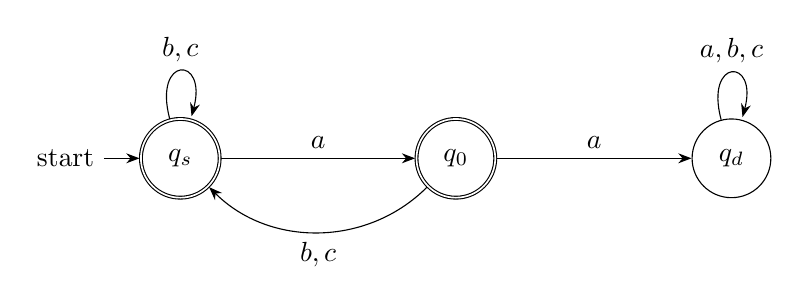
\begin{tikzpicture}[
    auto,
    >=Stealth
]

    % Estados
    \node[state, initial, accepting] (qs) at (0,0)   {$q_s$};
    \node[state, accepting]          (q0) at (3.5,0) {$q_0$};
    \node[state]                     (qd) at (7,0)   {$q_d$};

    % Transiciones
    \path[->]

        % Desde qs
        (qs)
            edge[loop above] node {$b,c$} ()
            edge node[above] {$a$} (q0)

        % Desde q0
        (q0)
            edge[bend left=45]
                node[below] {$b,c$} (qs)
            edge node[above] {$a$} (qd)

        % Estado muerto
        (qd)
            edge[loop above] node {$a,b,c$} ();

\end{tikzpicture}
\end{center}

\vspace{1cm}

% =========================================================
% EJERCICIO 18
% =========================================================

\section*{Exercise 18}

\begin{center}
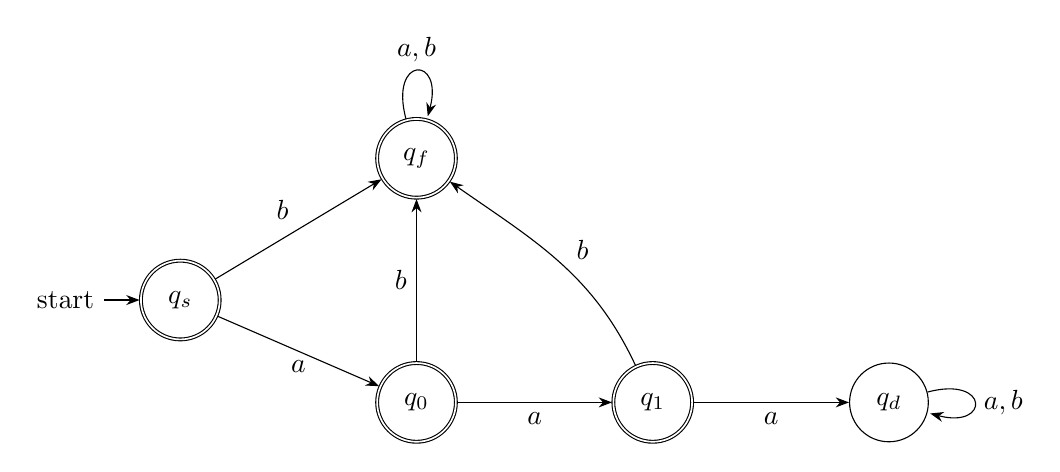
\begin{tikzpicture}[
    auto,
    >=Stealth
]

    % Estados
    \node[state, initial, accepting] (qs) at (0,0)      {$q_s$};

    \node[state, accepting]          (q0) at (3,-1.3)   {$q_0$};
    \node[state, accepting]          (q1) at (6,-1.3)   {$q_1$};

    % Estado seguro/final
    \node[state, accepting]          (qf) at (3,1.8)    {$q_f$};

    % Estado muerto
    \node[state]                     (qd) at (9,-1.3)   {$q_d$};

    % Transiciones
    \path[->]

        % Desde qs
        (qs)
            edge node[below] {$a$} (q0)
            edge node[above left] {$b$} (qf)

        % Desde q0
        (q0)
            edge node[below] {$a$} (q1)
            edge node[left] {$b$} (qf)

        % Desde q1
        (q1)
            edge node[below] {$a$} (qd)
            edge[
                out=115,
                in=-35
            ]
            node[pos=0.45, above right] {$b$} (qf)

        % Estado final seguro
        (qf)
            edge[loop above] node {$a,b$} ()

        % Estado muerto
        (qd)
            edge[loop right] node {$a,b$} ();

\end{tikzpicture}
\end{center}

\vspace{1cm}

% =========================================================
% EJERCICIO 19
% =========================================================

\section*{Exercise 19}

\begin{center}
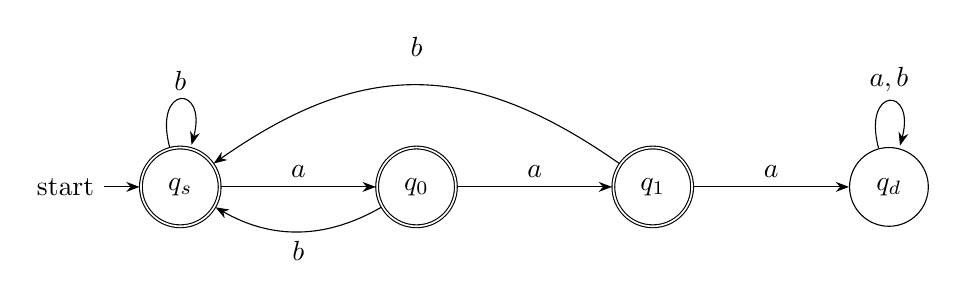
\begin{tikzpicture}[
    auto,
    >=Stealth
]

    % Estados
    \node[state, initial, accepting] (qs) at (0,0)   {$q_s$};
    \node[state, accepting]          (q0) at (3,0)   {$q_0$};
    \node[state, accepting]          (q1) at (6,0)   {$q_1$};
    \node[state]                     (qd) at (9,0)   {$q_d$};

    % Transiciones
    \path[->]

        % qs
        (qs)
            edge[loop above] node {$b$} ()
            edge node[above] {$a$} (q0)

        % q0
        (q0)
            edge node[above] {$a$} (q1)
            edge[bend left=30]
                node[below] {$b$} (qs)

        % q1
        (q1)
            edge node[above] {$a$} (qd)
            edge[
                out=145,
                in=35,
                looseness=1.15
            ]
            node[pos=0.5, above=7pt] {$b$} (qs)

        % Estado muerto
        (qd)
            edge[loop above] node {$a,b$} ();

\end{tikzpicture}
\end{center}

\vspace{1cm}

% =========================================================
% EJERCICIO 20
% =========================================================

\section*{Exercise 20}

\begin{center}
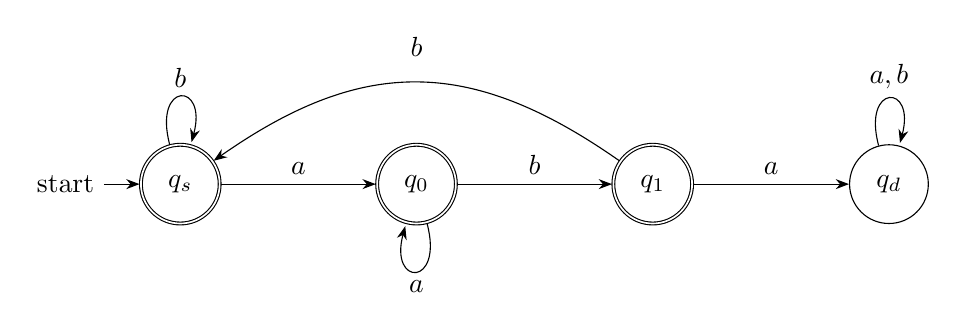
\begin{tikzpicture}[
    auto,
    >=Stealth
]

    % Estados
    \node[state, initial, accepting] (qs) at (0,0) {$q_s$};
    \node[state, accepting]          (q0) at (3,0) {$q_0$};
    \node[state, accepting]          (q1) at (6,0) {$q_1$};
    \node[state]                     (qd) at (9,0) {$q_d$};

    % Transiciones
    \path[->]

        % qs
        (qs)
            edge[loop above] node {$b$} ()
            edge node[above] {$a$} (q0)

        % q0
        (q0)
            edge[loop below] node {$a$} ()
            edge node[above] {$b$} (q1)

        % q1
        (q1)
            edge node[above] {$a$} (qd)
            edge[
                out=145,
                in=35,
                looseness=1.15
            ]
            node[pos=0.5, above=6pt] {$b$} (qs)

        % Estado muerto
        (qd)
            edge[loop above] node {$a,b$} ();

\end{tikzpicture}
\end{center}

\vspace{1cm}

% =========================================================
% EJERCICIO 21
% =========================================================

\section*{Exercise 21}

\begin{center}
\begin{tikzpicture}[
    auto,
    >=Stealth
]

    % Estados
    \node[state, initial]   (qs) at (0,0)      {$q_s$};
    \node[state]            (q0) at (3,0)      {$q_0$};

    \node[state, accepting] (q1) at (6,0)      {$q_1$};
    \node[state, accepting] (q2) at (6,-2.6)   {$q_2$};

    \node[state]            (qd) at (9,0)      {$q_d$};

    % Transiciones
    \path[->]

        % qs: todavía no aparece aa
        (qs)
            edge[loop above] node {$b$} ()
            edge node[above] {$a$} (q0)

        % q0: se acaba de leer una a
        (q0)
            edge[bend left=28]
                node[below] {$b$} (qs)
            edge node[above] {$a$} (q1)

        % q1: ya apareció aa exactamente una vez
        % y el último símbolo es a
        (q1)
            edge node[above] {$a$} (qd)
            edge node[right] {$b$} (q2)

        % q2: ya apareció aa una vez
        % y el último símbolo es b
        (q2)
            edge[loop below] node {$b$} ()
            edge[bend left=30]
                node[left] {$a$} (q1)

        % Estado muerto
        (qd)
            edge[loop right] node {$a,b$} ();

\end{tikzpicture}
\end{center}

\vspace{1cm}

% =========================================================
% EJERCICIO 22
% =========================================================

\section*{Exercise 22}

\begin{center}
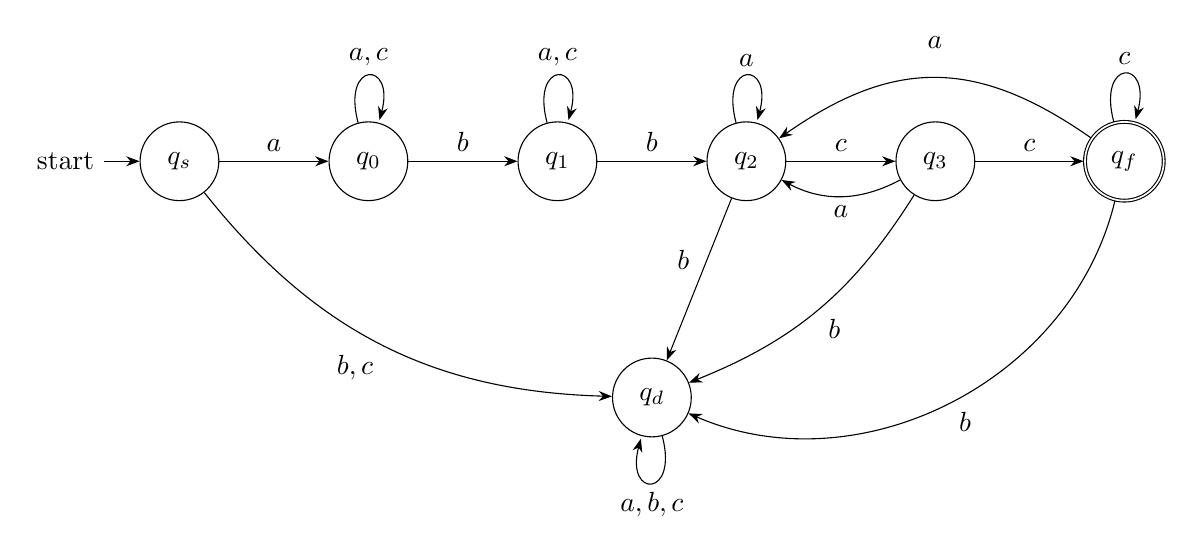
\begin{tikzpicture}[
    auto,
    >=Stealth
]

    % Estados
    \node[state, initial]   (qs) at (0,0)      {$q_s$};

    \node[state]            (q0) at (2.4,0)    {$q_0$};
    \node[state]            (q1) at (4.8,0)    {$q_1$};
    \node[state]            (q2) at (7.2,0)    {$q_2$};
    \node[state]            (q3) at (9.6,0)    {$q_3$};

    \node[state, accepting] (qf) at (12,0)     {$q_f$};

    \node[state]            (qd) at (6,-3)     {$q_d$};

    % Transiciones
    \path[->]

        % Estado inicial
        (qs)
            edge node[above] {$a$} (q0)
            edge[bend right=25]
                node[below left] {$b,c$} (qd)

        % Antes del primer b
        (q0)
            edge[loop above] node {$a,c$} ()
            edge node[above] {$b$} (q1)

        % Después del primer b
        (q1)
            edge[loop above] node {$a,c$} ()
            edge node[above] {$b$} (q2)

        % Ya aparecieron exactamente dos b
        (q2)
            edge[loop above] node {$a$} ()
            edge node[above] {$c$} (q3)
            edge node[above left] {$b$} (qd)

        % Se tiene un c al final
        (q3)
            edge node[above] {$c$} (qf)
            edge[bend left=28]
                node[below] {$a$} (q2)
            edge[bend left=18]
                node[below right] {$b$} (qd)

        % Se termina actualmente en cc
        (qf)
            edge[loop above] node {$c$} ()
            edge[
                out=145,
                in=35,
                looseness=1.15
            ]
            node[pos=0.5, above=7pt] {$a$} (q2)
            edge[bend left=50]
                node[below right] {$b$} (qd)

        % Estado muerto
        (qd)
            edge[loop below] node {$a,b,c$} ();

\end{tikzpicture}
\end{center}

\vspace{1cm}

% =========================================================
% EJERCICIO 23
% =========================================================

\section*{Exercise 23}

\begin{center}
\begin{tikzpicture}[
    auto,
    >=Stealth
]

    % Estados
    \node[state, initial]   (qs) at (0,0)      {$q_s$};

    % Rama superior
    \node[state]            (q0) at (2.8,1.7)  {$q_0$};
    \node[state]            (q1) at (5.6,1.7)  {$q_1$};

    % Rama inferior
    \node[state]            (q2) at (2.8,-1.7) {$q_2$};
    \node[state]            (q3) at (5.6,-1.7) {$q_3$};

    % Estado final
    \node[state, accepting] (qf) at (8.4,0)    {$q_f$};

    % Transiciones
    \path[->]

        % Desde qs
        (qs)
            edge node[above left] {$a$} (q0)
            edge node[below left] {$b$} (q2)

        % Rama superior
        (q0)
            edge[loop above] node {$a$} ()
            edge node[above] {$b$} (q1)

        (q1)
            edge[loop above] node {$b$} ()
            edge node[above right] {$a$} (qf)

        % Rama inferior
        (q2)
            edge[loop below] node {$b$} ()
            edge node[below] {$a$} (q3)

        (q3)
            edge[loop below] node {$a$} ()
            edge node[below right] {$b$} (qf)

        % Estado final
        (qf)
            edge[loop right] node {$a,b$} ();

\end{tikzpicture}
\end{center}

\vspace{1cm}

% =========================================================
% EJERCICIO 24
% =========================================================

\section*{Exercise 24}

\begin{center}
\begin{tikzpicture}[node distance=3cm, on grid, auto]

    % DFA Exercise 24

\end{tikzpicture}
\end{center}

\vspace{1cm}

% =========================================================
% EJERCICIO 25
% =========================================================

\section*{Exercise 25}

\begin{center}
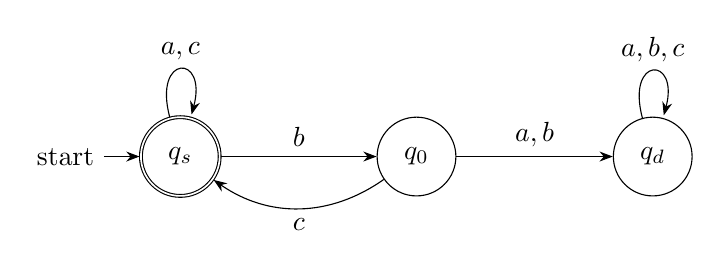
\begin{tikzpicture}[
    auto,
    >=Stealth
]

    % Estados
    \node[state, initial, accepting] (qs) at (0,0)   {$q_s$};
    \node[state]                     (q0) at (3,0)   {$q_0$};
    \node[state]                     (qd) at (6,0)   {$q_d$};

    % Transiciones
    \path[->]

        % Estado inicial / válido
        (qs)
            edge[loop above] node {$a,c$} ()
            edge node[above] {$b$} (q0)

        % Se acaba de leer b: obligatoriamente debe venir c
        (q0)
            edge[bend left=35]
                node[below] {$c$} (qs)
            edge node[above] {$a,b$} (qd)

        % Estado muerto
        (qd)
            edge[loop above] node {$a,b,c$} ();

\end{tikzpicture}
\end{center}

\vspace{1cm}

% =========================================================
% EJERCICIO 26
% =========================================================

\section*{Exercise 26}

\begin{center}
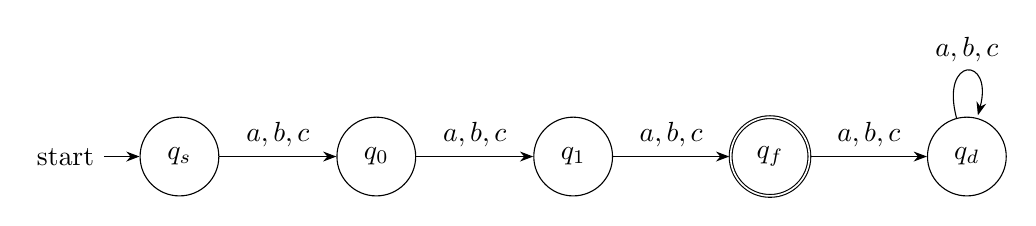
\begin{tikzpicture}[
    auto,
    >=Stealth
]

    % Estados
    \node[state, initial]   (qs) at (0,0)    {$q_s$};
    \node[state]            (q0) at (2.5,0)  {$q_0$};
    \node[state]            (q1) at (5,0)    {$q_1$};
    \node[state, accepting] (qf) at (7.5,0)  {$q_f$};
    \node[state]            (qd) at (10,0)   {$q_d$};

    % Transiciones
    \path[->]
        (qs)
            edge node[above] {$a,b,c$} (q0)

        (q0)
            edge node[above] {$a,b,c$} (q1)

        (q1)
            edge node[above] {$a,b,c$} (qf)

        (qf)
            edge node[above] {$a,b,c$} (qd)

        (qd)
            edge[loop above] node {$a,b,c$} ();

\end{tikzpicture}
\end{center}

\vspace{1cm}
% =========================================================
% EJERCICIO 27
% =========================================================

\section*{Exercise 27}

\begin{center}
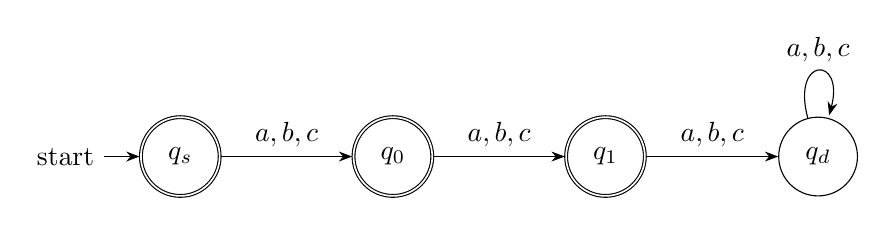
\begin{tikzpicture}[
    auto,
    >=Stealth
]

    % Estados
    \node[state, initial, accepting] (qs) at (0,0)    {$q_s$};
    \node[state, accepting]          (q0) at (2.7,0)  {$q_0$};
    \node[state, accepting]          (q1) at (5.4,0)  {$q_1$};
    \node[state]                     (qd) at (8.1,0)  {$q_d$};

    % Transiciones
    \path[->]

        (qs)
            edge node[above] {$a,b,c$} (q0)

        (q0)
            edge node[above] {$a,b,c$} (q1)

        (q1)
            edge node[above] {$a,b,c$} (qd)

        (qd)
            edge[loop above] node {$a,b,c$} ();

\end{tikzpicture}
\end{center}

\vspace{1cm}

% =========================================================
% EJERCICIO 28
% =========================================================

\section*{Exercise 28}

\begin{center}
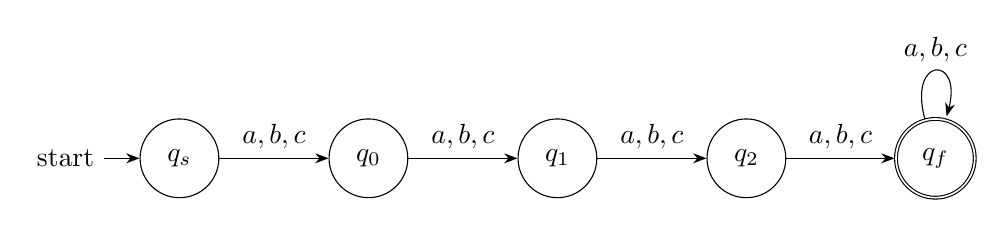
\begin{tikzpicture}[
    auto,
    >=Stealth
]

    % Estados
    \node[state, initial]   (qs) at (0,0)    {$q_s$};
    \node[state]            (q0) at (2.4,0)  {$q_0$};
    \node[state]            (q1) at (4.8,0)  {$q_1$};
    \node[state]            (q2) at (7.2,0)  {$q_2$};
    \node[state, accepting] (qf) at (9.6,0)  {$q_f$};

    % Transiciones
    \path[->]

        (qs)
            edge node[above] {$a,b,c$} (q0)

        (q0)
            edge node[above] {$a,b,c$} (q1)

        (q1)
            edge node[above] {$a,b,c$} (q2)

        (q2)
            edge node[above] {$a,b,c$} (qf)

        (qf)
            edge[loop above] node {$a,b,c$} ();

\end{tikzpicture}
\end{center}

\vspace{1cm}
% =========================================================
% EJERCICIO 29
% =========================================================

\section*{Exercise 29}

\begin{center}
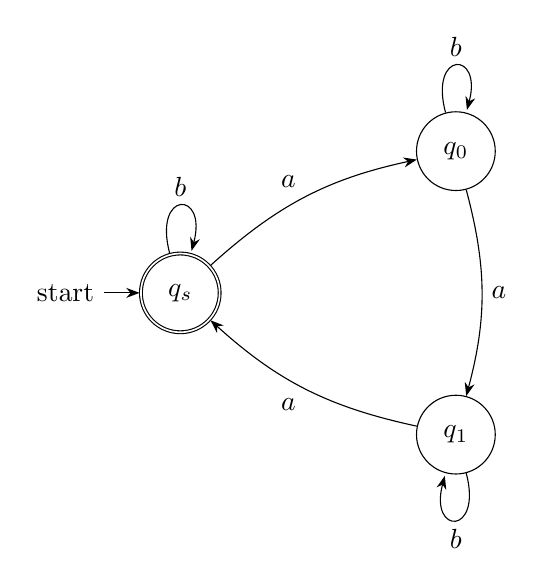
\begin{tikzpicture}[
    auto,
    >=Stealth
]

    % Estados
    \node[state, initial, accepting] (qs) at (0,0)     {$q_s$};
    \node[state]                     (q0) at (3.5,1.8) {$q_0$};
    \node[state]                     (q1) at (3.5,-1.8){$q_1$};

    % Transiciones
    \path[->]

        % q_s: 3k a's
        (qs)
            edge[loop above] node {$b$} ()
            edge[bend left=15] node[above left] {$a$} (q0)

        % q_0: 3k+1 a's
        (q0)
            edge[loop above] node {$b$} ()
            edge[bend left=15] node[right] {$a$} (q1)

        % q_1: 3k+2 a's
        (q1)
            edge[loop below] node {$b$} ()
            edge[bend left=15] node[below left] {$a$} (qs);

\end{tikzpicture}
\end{center}

\vspace{1cm}

% =========================================================
% EJERCICIO 30
% =========================================================

\section*{Exercise 30}

\begin{center}
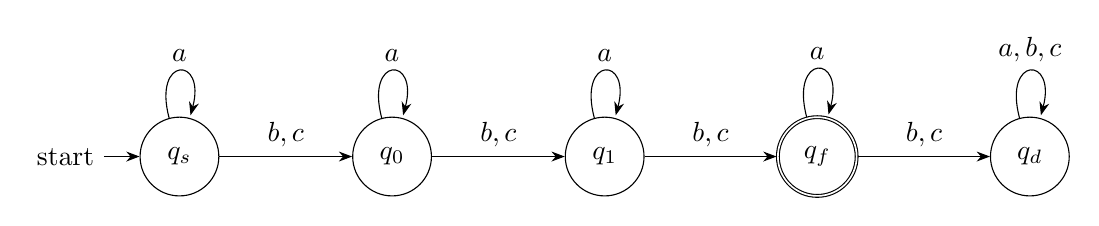
\begin{tikzpicture}[
    auto,
    >=Stealth
]

    % Estados
    \node[state, initial]   (qs) at (0,0)    {$q_s$};
    \node[state]            (q0) at (2.7,0)  {$q_0$};
    \node[state]            (q1) at (5.4,0)  {$q_1$};
    \node[state, accepting] (qf) at (8.1,0)  {$q_f$};
    \node[state]            (qd) at (10.8,0) {$q_d$};

    % Transiciones
    \path[->]

        % 0 ocurrencias de b o c
        (qs)
            edge[loop above] node {$a$} ()
            edge node[above] {$b,c$} (q0)

        % 1 ocurrencia de b o c
        (q0)
            edge[loop above] node {$a$} ()
            edge node[above] {$b,c$} (q1)

        % 2 ocurrencias de b o c
        (q1)
            edge[loop above] node {$a$} ()
            edge node[above] {$b,c$} (qf)

        % Exactamente 3 ocurrencias de b o c
        (qf)
            edge[loop above] node {$a$} ()
            edge node[above] {$b,c$} (qd)

        % Más de 3 ocurrencias
        (qd)
            edge[loop above] node {$a,b,c$} ();

\end{tikzpicture}
\end{center}

\vspace{1cm}

% =========================================================
% EJERCICIO 31
% =========================================================

\section*{Exercise 31}

\begin{center}
\begin{tikzpicture}[
    auto,
    >=Stealth
]

    % Estados
    \node[state, initial, accepting] (qs) at (0,0)      {$q_s$};
    \node[state, accepting]          (q0) at (3,1.8)    {$q_0$};
    \node[state]                     (q1) at (3,-1.8)   {$q_1$};
    \node[state]                     (qd) at (6,-1.8)   {$q_d$};

    % Transiciones
    \path[->]

        % Estado inicial / situación válida
        (qs)
            edge node[above left] {$b$} (q0)
            edge node[below left] {$a$} (q1)

        % Último símbolo fue b
        (q0)
            edge[loop above] node {$b$} ()
            edge[bend left=22]
                node[below right] {$a$} (qs)

        % a pendiente: necesita b inmediatamente después
        (q1)
            edge node[right] {$b$} (q0)
            edge node[above] {$a$} (qd)

        % Estado muerto
        (qd)
            edge[loop right] node {$a,b$} ();

\end{tikzpicture}
\end{center}

\vspace{1cm}

% =========================================================
% EJERCICIO 32
% =========================================================

\section*{Exercise 32}

\begin{center}
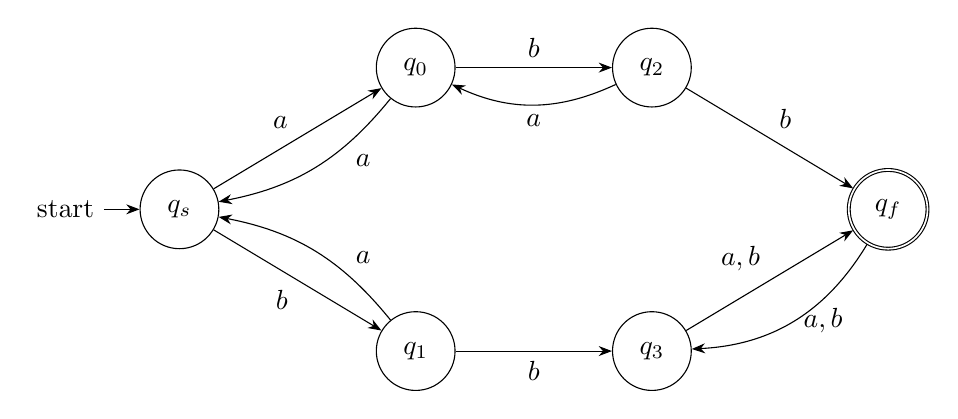
\begin{tikzpicture}[
    auto,
    >=Stealth
]

    % Estados
    \node[state, initial]   (qs) at (0,0)      {$q_s$};

    \node[state]            (q0) at (3,1.8)    {$q_0$};
    \node[state]            (q1) at (3,-1.8)   {$q_1$};

    \node[state]            (q2) at (6,1.8)    {$q_2$};
    \node[state]            (q3) at (6,-1.8)   {$q_3$};

    \node[state, accepting] (qf) at (9,0)      {$q_f$};

    % Transiciones
    \path[->]

        % q_s: longitud par, aún no aparece bb
        (qs)
            edge node[above left] {$a$} (q0)
            edge node[below left] {$b$} (q1)

        % q0: longitud impar, último símbolo no es b
        (q0)
            edge[bend left=20]
                node[below right, pos=0.3] {$a$} (qs)
            edge node[above] {$b$} (q2)

        % q1: longitud impar, último símbolo es b
        (q1)
            edge[bend right=20]
                node[above right, pos=0.3] {$a$} (qs)
            edge node[below] {$b$} (q3)

        % q2: longitud par, último símbolo es b, aún sin bb
        (q2)
            edge[bend left=25]
                node[below] {$a$} (q0)
            edge node[above right] {$b$} (qf)

        % q3: ya apareció bb y la longitud es par
        (q3)
            edge node[above left] {$a,b$} (qf)

        % qf: ya apareció bb y la longitud es impar
        (qf)
            edge[bend left=28]
                node[right] {$a,b$} (q3);

\end{tikzpicture}
\end{center}

\vspace{1cm}

% =========================================================
% EJERCICIO 33
% =========================================================

\section*{Exercise 33}

\begin{center}
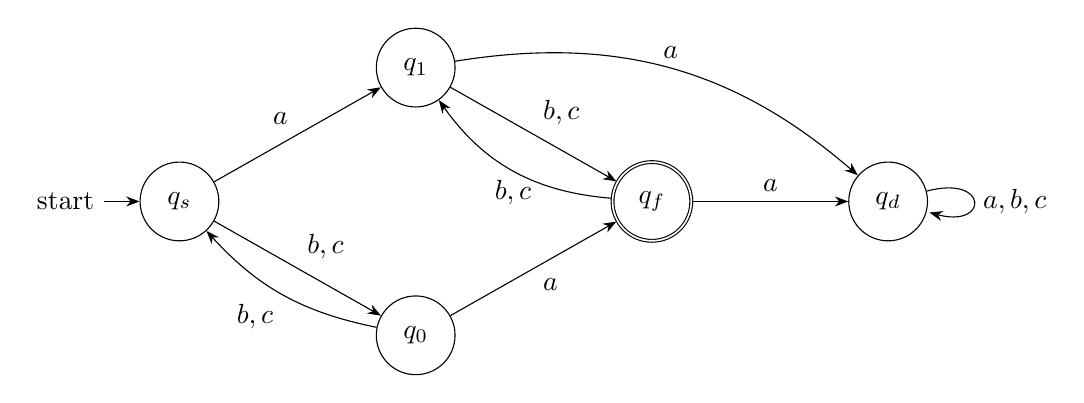
\begin{tikzpicture}[
    auto,
    >=Stealth
]

    % Estados
    \node[state, initial]   (qs) at (0,0)       {$q_s$};

    \node[state]            (q1) at (3,1.7)     {$q_1$};
    \node[state]            (q0) at (3,-1.7)    {$q_0$};

    \node[state, accepting] (qf) at (6,0)       {$q_f$};

    \node[state]            (qd) at (9,0)       {$q_d$};

    % Transiciones
    \path[->]

        % q_s: longitud par, 0 a's
        (qs)
            edge node[above left] {$a$} (q1)
            edge node[above right] {$b,c$} (q0)

        % q_0: longitud impar, 0 a's
        (q0)
            edge[bend left=18]
                node[below left] {$b,c$} (qs)
            edge node[below right] {$a$} (qf)

        % q_1: longitud impar, exactamente una a
        (q1)
            edge node[above right] {$b,c$} (qf)
            edge[bend left=25]
                node[above] {$a$} (qd)

        % q_f: longitud par, exactamente una a
        (qf)
            edge[bend left=25]
                node[below] {$b,c$} (q1)
            edge node[above] {$a$} (qd)

        % Estado muerto: dos o más a's
        (qd)
            edge[loop right] node {$a,b,c$} ();

\end{tikzpicture}
\end{center}

\vspace{1cm}

% =========================================================
% EJERCICIO 34
% =========================================================

\section*{Exercise 34}

\begin{center}
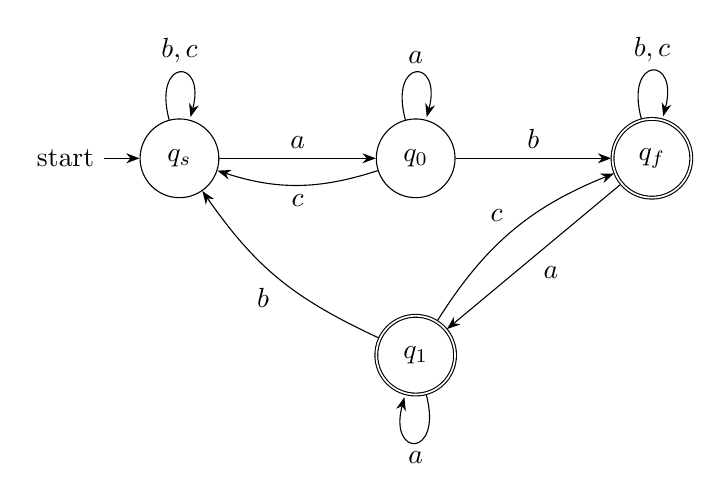
\begin{tikzpicture}[
    auto,
    >=Stealth
]

    % Estados
    \node[state, initial]   (qs) at (0,0)       {$q_s$};
    \node[state]            (q0) at (3,0)       {$q_0$};

    \node[state, accepting] (qf) at (6,0)       {$q_f$};
    \node[state, accepting] (q1) at (3,-2.5)    {$q_1$};

    % Transiciones
    \path[->]

        % Par de ocurrencias de ab,
        % último símbolo distinto de a
        (qs)
            edge[loop above] node {$b,c$} ()
            edge node[above] {$a$} (q0)

        % Par de ocurrencias de ab,
        % último símbolo es a
        (q0)
            edge[loop above] node {$a$} ()
            edge[bend left=18]
                node[below] {$c$} (qs)
            edge node[above] {$b$} (qf)

        % Impar de ocurrencias de ab,
        % último símbolo distinto de a
        (qf)
            edge[loop above] node {$b,c$} ()
            edge node[below right] {$a$} (q1)

        % Impar de ocurrencias de ab,
        % último símbolo es a
        (q1)
            edge[loop below] node {$a$} ()
            edge[bend left=18]
                node[above left] {$c$} (qf)
            edge[
                out=155,
                in=-55,
                looseness=1.05
            ]
            node[pos=0.5, below left] {$b$} (qs);

\end{tikzpicture}
\end{center}

\vspace{1cm}

% =========================================================
% EJERCICIO 35
% =========================================================

\section*{Exercise 35}

\begin{center}
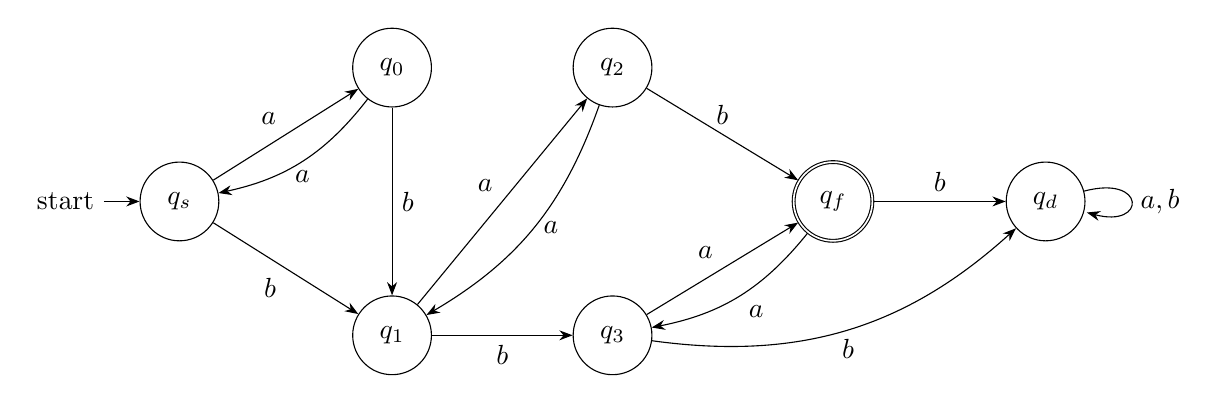
\begin{tikzpicture}[
    auto,
    >=Stealth
]

    % Estados
    \node[state, initial]   (qs) at (0,0)       {$q_s$};

    % 0 b's
    \node[state]            (q0) at (2.7,1.7)   {$q_0$};

    % 1 b
    \node[state]            (q1) at (2.7,-1.7)  {$q_1$};
    \node[state]            (q2) at (5.5,1.7)  {$q_2$};

    % 2 b's
    \node[state]            (q3) at (5.5,-1.7)   {$q_3$};
    \node[state, accepting] (qf) at (8.3,0)     {$q_f$};

    % Más de 2 b's
    \node[state]            (qd) at (11,0)      {$q_d$};

    % Transiciones
    \path[->]

        % q_s: 0 b, longitud par
        (qs)
            edge node[above left] {$a$} (q0)
            edge node[below left] {$b$} (q1)

        % q_0: 0 b, longitud impar
        (q0)
            edge[bend left=20]
                node[below] {$a$} (qs)
            edge node[right] {$b$} (q1)

        % q_1: 1 b, longitud impar
        (q1)
            edge node[above left] {$a$} (q2)
            edge node[below] {$b$} (q3)

        % q_2: 1 b, longitud par
        (q2)
            edge[bend left=20]
                node[right] {$a$} (q1)
            edge node[above] {$b$} (qf)

        % q_3: 2 b, longitud par
        (q3)
            edge node[above left] {$a$} (qf)
            edge[bend right=25]
                node[below] {$b$} (qd)

        % q_f: 2 b, longitud impar
        (qf)
            edge[bend left=20]
                node[below right] {$a$} (q3)
            edge node[above] {$b$} (qd)

        % q_d: más de 2 b's
        (qd)
            edge[loop right] node {$a,b$} ();

\end{tikzpicture}
\end{center}

\vspace{1cm}

% =========================================================
% EJERCICIO 36
% =========================================================

\section*{Exercise 36}

\begin{center}
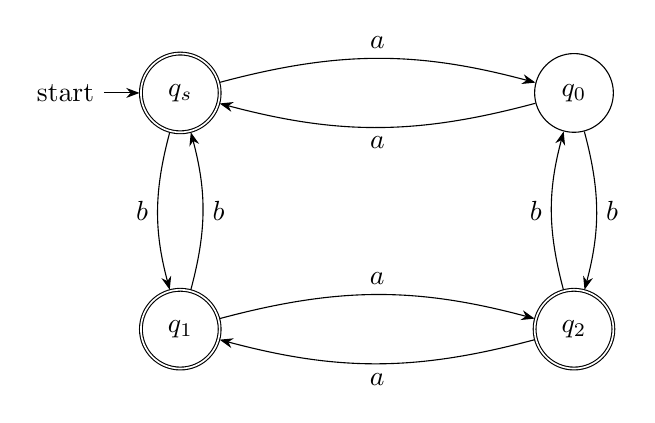
\begin{tikzpicture}[
    auto,
    >=Stealth
]

    % Estados
    % q_s: a par, b par
    \node[state, initial, accepting] (qs) at (0,2.5) {$q_s$};

    % q_0: a impar, b par
    \node[state]                     (q0) at (5,2.5) {$q_0$};

    % q_1: a par, b impar
    \node[state, accepting]          (q1) at (0,-0.5) {$q_1$};

    % q_2: a impar, b impar
    \node[state, accepting]          (q2) at (5,-0.5) {$q_2$};

    % Transiciones
    \path[->]

        % Fila superior: leer a cambia la paridad de a
        (qs)
            edge[bend left=15]
                node[above] {$a$} (q0)

        (q0)
            edge[bend left=15]
                node[below] {$a$} (qs)

        % Fila inferior
        (q1)
            edge[bend left=15]
                node[above] {$a$} (q2)

        (q2)
            edge[bend left=15]
                node[below] {$a$} (q1)

        % Columna izquierda: leer b cambia la paridad de b
        (qs)
            edge[bend right=15]
                node[left] {$b$} (q1)

        (q1)
            edge[bend right=15]
                node[right] {$b$} (qs)

        % Columna derecha
        (q0)
            edge[bend left=15]
                node[right] {$b$} (q2)

        (q2)
            edge[bend left=15]
                node[left] {$b$} (q0);

\end{tikzpicture}
\end{center}
\vspace{1cm}

\end{document}